\section{Artificial Neural Network} \label{neuralnetwork}  
As mentioned in \textbf{\autoref{sec:scene_analysis}}, neural networks are organised into several layers, known as the \textit{input layer}, the \textit{hidden layer} and the \textit{output layer}, which are depicted in \textbf{\autoref{fig:ann}}. As the names suggest, the input layer takes the external data as input to the \gls{ann}, and the output layer outputs the computational results. A training phase is used to learn the datasets to assign weights to the neurons in the neural network based on error rates between the target output and actual output.\cite{SAIRAMYA2019253} To train an \gls{ann}, backpropagation and Gradient Descent is used to improve the performance of the model\cite{SAIRAMYA2019253, ann}.

\begin{figure}[H]
    \centering
    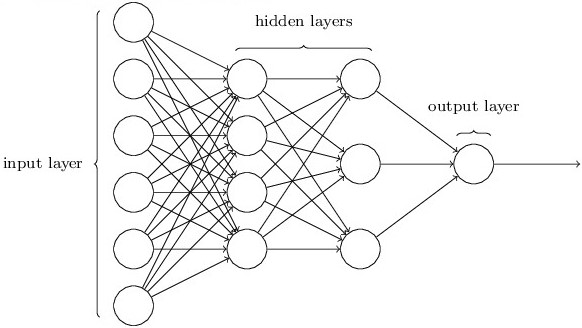
\includegraphics[scale=0.75]{Images/Experiments/ann_architecture.jpg}
    \caption{Four-layer neural network\cite{ann}.}
     \label{fig:ann}
\end{figure}

\subsection{Forward Propagation}
The phase of propagating an input vector through the network and getting an output is called \textit{forward propagation}. The \gls{ann} takes a vector as input which is passed to the input layer in \textbf{\autoref{fig:ann}}. The network can have one or several hidden layers after the input layer, each layer containing neurons. To get the output of a layer, the neurons or weights are multiplied by the input, and an activation function is applied to the result of the aforementioned computation.
%The number of neurons in the output layer equals the number of possible classifications.
The output of the output layer will be the final prediction made by the \gls{ann}.\cite{ann} An activation function is applied in the layers of the \gls{ann} to introduce non-linearity to make the model fit better to the data. Without non-linear activation functions, several hidden layers do not make sense, as they do not add additional power compared to a single layer. Non-linear activation function also makes it possible to non-linearly map the input to the output, which is necessary for most real world application.%, which is also the reason for the \gls{ann} being called the universal function approximator. 
%to represent the value given by the node as preferred\cite{nnadl}. In this example, the node output is a probability. That is, a value between 0 and 1.
In the \gls{ann}, the output of the previous layer is given an input to the next layer, while the output of the output layer is the final prediction.\cite{ann}%, known as \textit{feedforward} neural networks, where cycles are not allowed as in \textit{recurrent} neural networks.\cite{ann}

\subsection{Backpropagation}
The backpropagation algorithm is used for understanding how much the weights in a network contributes to the loss. The backpropagation algorithm is used to find the gradient of the cost function, which includes the magnitude and direction of the function. The algorithm uses the chain rule of differential calculus, which will compute the error gradient through summations of the local-gradient product over the different paths in the network from a node to the output. %This calculation can be done efficiently using dynamic programming, and the backpropagation algorithm is an application of dynamic programming. 

%The backpropagation includes two main phases: the forward phase and the backward phase.

The backpropagation includes two main steps: the forward pass to calculate loss and a backtracking step, which traverses backwards from the deeper layers to calculate the derivatives of the weights, with respect to the loss. The forward pass is calculated through forward propagation.
%In the forward phase, the training data is fed to the neural network, and a cascade of computations will happen throughout the layers using the current weights. The output from the training will be compared to the final predicted output, and the derivative of the loss function is computed. 
In the backwards phase, the goal is to use the chain rule to compute the gradient of the loss function, with respect to the different weights of the network. The gradients can thereafter be used to update the weights through gradient descent, explained in the following section. In this way, we optimize the weights, so the neural network will gain knowledge of how to correctly map the inputs to the outputs of the neural network.\cite{nnadl}

\subsection{Gradient Descent}
Gradient Descent is an algorithm that updates weights and biases for neurons so that the output from the neural network approximates its prediction for all training inputs. The main idea is to find the weights and biases so that the cost is as small as possible. Minimising the cost makes it easier to change the weights and biases in order to improve performance compared to maximizing the number of correct detection outputs.\cite{ann}

We let cost be a function defined as $C(v)$, where $v$ is a set of many variables. We can minimise the function $C(v)$ by finding where $C$, in the optimal case, achieves its global minimum. We find the minimum by computing derivatives of $C$, since this would tell us the slopes of the function, which in turn tells the minimum of $C$.\cite{ann}